\documentclass[12pt,oneside,a4paper,bibtotoc,liststotoc]{scrreprt}
\usepackage{remreset}

%% Listings
\usepackage{listings}
\lstset{
  basicstyle=\footnotesize, 
  stringstyle=\ttfamily,
  frame=single,
  numberbychapter=false, % Listings vom Anfang bis zum Ende
                         % durchnummerieren
  captionpos=b
}
% Fußnoten, Tabellen und Grafiken von Anfang bis Ende durchnummerieren.
\usepackage{chngcntr}
\counterwithout{footnote}{chapter}
\counterwithout{table}{chapter}
\counterwithout{figure}{chapter}

% Überschriften bis zur dritten Ebene durchnummerieren
\setcounter{secnumdepth}{3}
% Überschriften bis zur zweiten Ebene in den TOC
\setcounter{tocdepth}{2}

%% Typographie-Schnickschnack
\usepackage[T1]{fontenc}
\usepackage{lmodern}
\usepackage{ellipsis} 

%% Absatzformatierung
% \parindent=0cm
\parskip=3mm

% Schönere Zeilenumbrüche
\usepackage{microtype}
\tolerance 1414
\hbadness 1414
\emergencystretch 1.5em
\hfuzz 0.3pt
\vfuzz \hfuzz
\raggedbottom
% Schusterjungen und Hurenkinder unterdrücken
\clubpenalty = 10000 
\widowpenalty = 10000 
\displaywidowpenalty = 10000 
% Schuster- und Hurenfußnoten will auch keiner...
\interfootnotelinepenalty=10000 

\usepackage[utf8]{inputenc}
% Mathematischen Formelsatz erlauben
\usepackage{amsmath}
\usepackage{amssymb}
\usepackage[ngerman]{babel}

%% Wenn ein Index verwendet werden soll, folgendes auskommentieren
% \usepackage{makeidx}
% \makeindex

\usepackage{graphicx}

% Erlaube das Setzen von anderne Zeilenabständen (s.u.)
\usepackage{setspace} 

%% Literaturverzeichnis
\usepackage{jurabib}
\jurabibsetup{
	authorformat=abbrv,
        titleformat={short,commasep},
	commabeforerest,
	see,
%        super, %% Konvertiert alle \cite in \footcite
        square,
%        citefull=first,
}
% Typographischer Schnickschnack für Bibliographie
\renewcommand*{\jbauthorfont}{\textsc}
\renewcommand*{\biblnfont}{\scshape\textbf}
\renewcommand*{\bibfnfont}{\normalfont\textbf}

%% % Abstand vor Kapitelüberschriften: 0 cm (um es Bündig zu setzen, negativen Skip verwenden)
\renewcommand*{\chapterheadstartvskip}{\vspace*{0cm}}
%% % Abstand nach Kapitelüberschriften: 1 Zeile
\renewcommand*{\chapterheadendvskip}{\vspace{1\baselineskip}}

% Referenzen verlinken
\usepackage{hyperref}
\hypersetup{ 
    colorlinks,
    citecolor=black,
    filecolor=black,
    linkcolor=black,
    urlcolor=black 
}

% Grad-Zeichen definieren
\newcommand{\grad}{\mbox{\(\mathsurround=0pt{}^\circ\)}}
% (r)-Zeichen definieren
\def\TReg{\textsuperscript{\textregistered}}
% z.B., d.h. usw. Typographisch korrekt setzen
\usepackage{xspace}
\newcommand{\zB}{\mbox{z.\,B.}\xspace}
\newcommand{\dH}{\mbox{d.\,h.}\xspace}
\newcommand{\ua}{\mbox{u.\,a.}\xspace}
\newcommand{\so}{\mbox{s.\,o.}\xspace}
\newcommand{\MSc}{\mbox{M.\,Sc.}\xspace}
\newcommand{\BSc}{\mbox{B.\,Sc.}\xspace}


%% Schönere Tabellen
\usepackage{booktabs}
\usepackage{tabularx}

%% Ränder setzen
\usepackage[left=5cm,right=3cm,top=1.5cm,bottom=2cm,includeheadfoot]{geometry}

%% Abkürzungsverzeichnis
\usepackage[printonlyused]{acronym}

%% Allow really fixed positions for Tables
\usepackage{float}
\restylefloat{table}

%% Gedrehte Tabellen
\usepackage{rotating}

%% Trennung tweaken: Manche Wörter will man ggf. anders trennen als
%% der Algorithmus das vorsieht oder ggf. auch garnicht
\hyphenation{Java-Script}
\hyphenation{Cookies}

\begin{document}
\begin{titlepage} 
\begin{figure}[H]
  \begin{flushright}
    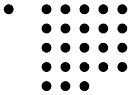
\includegraphics{img/fh-koeln-logo.png}
    \label{logo_fh_köln}
  \end{flushright}
\end{figure}

\begin{center}
\textbf{\Large\newline  Fachhochschule Köln\\
Cologne University of Applied Sciences\\[0.1cm]
\normalsize Campus Gummersbach\\
Fakultät für Informatik und Ingenieurwissenschaften\\[0.5cm]}

 
\Large Verbundstudiengang Wirtschaftsinformatik\\[0.5cm]

\large Masterthesis\\[0.1cm]
  
% Title
{ \huge \bfseries \ Konzepte der Nebenläufigkeit  \\[0.1cm]
        unter Android \\[0.5cm]
        
}
\vfill

\begin{table}[h]
\centering
\begin{tabular}{ll}
  Prüfer:         & Prof. Dr. Erich Ehses \\
  Zeitprüfer:     & Prof. Dr. Frank Victor \\
  vorgelegt am:   & \today \\
  von cand.:      & Stephan Wagner \\
  aus:            & Overath \\
  Telefon-Nr.:    & +49-176-80007570 \\
  Matrikel-Nr.:   & 1106011828 \\
  E-Mail-Adresse: & stephan.wagner.mi738@gmail.com
\end{tabular}
\end{table}
\end{center}
\end{titlepage}



\onehalfspacing % 1,5-facher Zeilenabstand

\chapter*{Zusammenfassung}
Diese Thesis behandelt das Thema „Konzepte der Nebenläufigkeit unter Android“. Darin wird zunächst als Einführung in die Thematik, die Nebenläufigkeit allgemein mit ihren unterschiedlichen Ausprägungen (Prozess-/Threadebene) erläutert und die Risiken die mit Nebenläufigkeit einhergeht skizziert. Dabei ist ein besonders wichtiger Punkt der Botschaftenaustausch, der mittels unterschiedlicher Techniken realisierbar ist. Auch hier birgt jede Technologie ihre individuellen Vor- und Nachteile.
Die Nebenläufigkeit unter Android unterliegt einigen Besonderheiten, die sich teilweise aus den Restriktionen des Betriebssystems ergeben, aber auch aus den Anforderungen für die Android Applikationsentwicklung, die der StyleGuide vorgibt. So ist die grundsätzliche Anforderung, dass Applikationen ansprechbar bleiben. Eine Applikation, insbesondere eine Gui Applikation sollte somit beim Start von Operationen weder blockieren oder nicht mehr auf Benutzereingaben reagieren. Technisch bedeutet dies, dass zeitaufwändige Operationen nie auf dem Main Thread der Applikation stattfinden dürfen. Stattdessen müssen derartige Operationen in Hintergrundthreads ausgelagert werden. Im Kapitel 2 werden hierzu drei unterschiedliche Konzepte an Hand konkreten Beispielimplementierungen vorgestellt und in der jeweiligen Funktionsweise analysiert.
\begin{itemize}
\item Java Concurrency nach Java SE
\item Android Concurrency aus dem Android SDK
\item RXJava Framework
\end{itemize}
Die aus der technischen Analyse gewonnenen Erkenntnisse werden in Kapitel 3 genutzt um Chancen und Risiken der einzelnen Konzepte zu diskutieren. Um die Ergebnisse aus dem Diskurs für zukünftige Entscheidungsfindungen zu Rate ziehen zu können fließen die aus der Detailanalyse gewonnenen Ergebnisse in eine Szenarien basierte Analyse ein, um daraus Anhaltspunkte für den sinnvollen Einsatz der Konzepte abzuleiten.

\tableofcontents
\listoffigures


\chapter{Einleitung}
\section{Motivation}
Mobile Endgeräte begleiten immer mehr Menschen in ihrem Alltag. Damit einher geht die intensive Nutzung von sog. Apps., womit Applikationen auf den mobilen Endgeräten bezeichnet werden. Mit der zunehmenden Leistungsfähigkeit der Geräte werden auch immer komplexere Applikationen realisierbar. Wurde zu den Anfängen der Applikationsentwicklung für mobile Endgeräte lediglich einfache Funktionalität in Applikationen integriert, werden heute mit unter teilweise sehr rechenintensive und komplexe Funktionalitäten entwickelt. Eine optimale Konzeption der Aufgabenverarbeitung innerhalb der Applikation kann dabei einen entscheidenden Faktor für die Performance und damit auch die Akzeptanz beim Nutzer darstellen. Damit gewinnt die Nebenläufigkeit auch in der Applikationsentwicklung für mobile Endgeräte an Wichtigkeit. Nebenläufigkeit oder auch Parallelverarbeitung bezeichnet in der Informatik die Eigenschaft eines Programms oder eines Systems verschiedene Aufgaben zeitgleich, also parallel zu bearbeiten. Die jeweilige Verarbeitung kann dabei in sich abgeschlossen sein, d.h. die zu verarbeitenden Aufgaben sind voneinander unabhängig, oder die Verarbeitung hängt von den Ergebnissen aus anderen Aufgaben ab. Je nach Art und Weise der Parallelverarbeitung sind verschiedene Problematiken und Risiken zu beachten. Für Nebenläufigkeit unter dem Android Betriebssystem sind zusätzliche Besonderheiten zu beachten. Dieses Betriebssystem ist auf mobile Endgeräte zugeschnitten und hat diesbezüglich spezielle Anforderungen an Applikationen die darauf laufen sollen. Die Firma Google als Hersteller vom Betriebssystem Android legt hierbei großen Wert auf die Einhaltung eines StyleGuides der die Benutzbarkeit applikationsübergreifend in einem einheitlichen Standard definiert. Darin wird die grundlegende Anforderung nach der kontinuierlichen Ansprechbarkeit von Applikationen gefordert. Die Frage ist wie kann den Anforderungen an Android Applikationen mittels unterschiedlicher Konzepte der Nebenläufigkeit begegnet werden, sodass das von Google geforderte Ziel der Ansprechbarkeit erreicht werden kann. Welche Problemstellungen, Restriktionen oder Risiken gehen mit der Verwendung bestimmter Konzepte einher und wie praktikabel sind diese für den konkreten Praxiseinsatz? 

\section{Zielsetzung und Vorgehen}
In dieser Arbeit soll untersucht werden, wie konkurrierende Parallelverarbeitung in mobilen Anwendungen realisiert werden kann. Dabei besteht das Ziel, die Entwicklung von Nebenläufigkeit durch Verwendung unterschiedlicher Techniken zu vereinfachen und ggf. auf einem höheren Abstraktionsniveau ab zu bilden. Zunächst gilt es in einer kurzen Einführung in die Thematik, die grundsätzlichen Definitionen kurz zu erläutern und auf Besonderheiten der Parallelverarbeitung unter Android einzugehen. Weiter wird ein Überblick über eine Auswahl von unterschiedlichen Konzepten der Nebenläufigkeit unter Android erarbeitet. Diese werden mittels einfacher Beispiele vorgestellt und analysiert. Den Abschluss bildet ein kritischer Diskurs, um in Abhängigkeit vom Einsatzkontext eine Differenzierte Sicht auf die Anwendung der einzelnen Konzepte zu erhalten. Die Ergebnisse des Diskurses werden in einer szenarienbasierten Analyse aufgegriffen um diese greifbarer zu machen.

\section{Begriffsdefinition und Grundlagen der Nebenläufigkeit}
Um sich den Konzepten der Nebenläufigkeit anzunähern, werden zunächst einige Begriffsdefinitionen benötigt. Die Nebenläufigkeit meint dabei konkret die parallele Verarbeitung von Aufgaben. Hierzu wird eine Aufgabe in Unteraufgaben aufgeteilt, um diese  weitestgehend von einander unabhängig abzuarbeiten. Die Definition wie diese Verarbeitung ablaufen soll, ist in einem Programm hinterlegt. Die Ausführung von Programmen wird von Prozessen und Threads geregelt. Diese werden im folgenden Abschnitt definiert und ein tieferes Verständnis von der Parallelverarbeitung auf Betriebssystemebene erarbeitet.

\section{Prozesse und Threads}
Die genauen Eigenschaften von Prozessen und Threads sind abhängig vom Betriebssystem auf dem sie laufen. Da in dieser Arbeit der Fokus auf Nebenläufigkeit unter Android liegt, beziehen sich die folgenden Erläuterungen zu Prozessen und Threads auf das allgemeine Unix/Linux Betriebssystem auf dem Android basiert.

\subsection{Prozess}
Wird eine Anwendung gestartet, so erzeugt das Betriebssystem zunächst einen Prozess, der den Adressraum für sämtliche Programmdaten und Komponenten reserviert. Für Prozesse kann folgende Definition getroffen werden. Sie gilt betriebssystemübergreifend:
\begin{center}
Ein Prozess stellt ein Programm in Ausführung dar und
ist für die Kontrolle(Sicherung) der damit verbundenen Betriebsmittel
verantwortlich.
\end{center}
Die Prozesse sind (in der Regel) an einen Benutzer gebunden, welcher wiederum über bestimme Rechte u.a. im Dateisystem verfügt. Dabei sind für Linux Betriebssysteme folgende Prinzipien zu beachten:
\begin{itemize}
\item Hierarschische Prinzip
\item Sandbox Prinzip
\end{itemize}
Das hierarchische Prinzip schreibt die Abhängigkeit von Prozessen gegenüber ihren Erzeugern vor. Mit Ausnahme des Root Prozesses des Betriebssystems, werden alle Anwendungen durch einen Vater Prozess erzeugt. Die damit verbundene Vater-Kind Abhängigkeit bildet eine Baumstruktur, in der jeder Prozess seinen erzeugenden Prozess kennt. Ein Prozess kann nur aus anderen Prozessen heraus erzeugt werden. Stirbt ein Prozess, so werden die Kind Prozesse in der Regel vom Root Prozess des Betriebsystems adoptiert.\newline
Das Sandbox Prinzip ist ein Sicherheitskonzept aus dem Kern eines Linux/Unix Betriebssystems. Darin wird sichergestellt, dass jede Anwendung nur die eigenen Daten sehen darf. So wird bei der Installation für jede Anwendung ein eigener Betriebssystem- User erzeugt, der über spezielle Rechte zu Prozessen und Dateien verfügt. Damit wird zum Ausführungszeitpunkt verhindert, dass Programmdaten für andere Programme sichtbar werden. Die Sicht jedes Prozesses einer Anwendung ist begrenzt auf die Ressourcen die dem jeweiligen Betriebssystem User zugeordnet sind.

\subsection{Thread}
Die Begriffe Prozesse und Threads dürfen nicht synonym verwendet werden. So kann ein Thread wie folgend Definiert werden:
\begin{center}
Ein Thread stellt einen Ausführungsfaden
eines Programmes dar.
\end{center}
Dieser besteht aus aus einem aktuellen Befehlszeiger, einem eigenen Stack und dem Inhalt der Prozessorregister. Zum Start einer Anwendung wird der sog. Main Thread erzeugt. Aus diesem lassen sich beliebig weitere Threads erzeugen. Dabei besteht keine hierarchische Bindung wie bei der Vater-Sohn Prozesshierarchie. Innerhalb eines Prozesses erzeugte Threads erhalten Zugriff auf den hier reservierten Speicher des Prozesses. Alle in einem Prozess erzeugte Threads sind von diesem abhängig. Wird demnach ein Prozess terminiert, so werden auch alle darin erzeugte Threads terminiert.

\section{Botschaftenaustausch und Kommunikation}
Der Botschaftenaustausch zwischen Prozessen unterscheidet sich vom Botschaftenaustausch zwischen Threads. Während bei der Inter Prozess Kommunikation maßgeblich das Betriebssystem am Austausch von Nachrichten zwischen Prozessen beteiligt ist, können bei der Inter Thread Kommunikation unterschiedliche Techniken unabhängig vom Betriebssystem angewandt werden. Für die Kommunikation zwischen Threads eignen sich z.B. Dateien aber auch sogenannte MessageQueues mit denen Produzenten und Konsumenten Konstrukte erzeugt werden können. Die Inter Thread Kommunikation bleibt begrenzt auf die Threads innerhalb einer Anwendung. Die Inter Prozess Kommunikation dagegen, definiert die Kommunikation über Programm- und Systemgrenzen hinaus. Innerhalb eines Betriebssystems wird in der Regel der Speicherbereich jedes Prozesses in sich gekapselt und vor anderen Prozessen verborgen (s.o. Sandbox-Prinzip). Daher werden Mechanismen seitens des Betriebssystems benötigt (Botschaftenaustausch über Socket, etc..) um die Kommunikation zu gewährleisten. Diese Mechanismen sind aufwendig und eignen sich dadurch weniger für eine effiziente Parallelverarbeitung. Daher konzentriert sich diese Arbeit auf die Kommunikation auf Thread Ebene, und die Inter Prozess Kommunikation wird nicht weiter thematisiert. Die folgenden Abschnitte geben einen Einblick auf gängige Techniken zur Realisierung von Inter Thread Kommunikation.

\subsection{Geteilte Datei/ Speicher}
Einer der einfachsten technischen Mittel für den Daten- /Botschaftenaustauch ist die Nutzung einer gemeinsamen Datei im Dateisystem des Betriebssystems. Dadurch, dass das Betriebssystem den exklusiven Zugriff auf Dateien gewährleisten kann, ist es möglich ohne großen Aufwand eine synchronisierte Kommunikation zu realisieren. Etwas komplexer ist es für die Kommunikation einen Speicherbereich zu allokieren und die Referenz darauf den jeweiligen Kommunikationspartern für den Datenaustausch zur Verfügung zu stellen. In diesem Fall muss der exklusive Ausschluss selbst realisiert werden, falls er gewünscht ist. Hierzu dienen einfache Primitive aus dem java.lang.concurrency Packet.

\subsection{MessageQueues}
Die folgende Abbildung gibt einen schematischen Überblick über die Nutzung einer MessageQueue für die Kommunikation zwischen Objektinstanzen aus unterschiedlichen Threads. Beide Objekt Instanzen müssen eine Referenz auf das MessageQueue Objekt halten um Nachrichten (z.B. Message to Thread B) in diese Queue einzustellen oder herauszuholen. Das Konzept des nachrichtengetriebenen Datenaustausches hat den Vorteil, dass jede Nachricht eine atomare (in sich geschlossene) Einheit darstellt. Dadurch lassen sich einzelne Arbeitsaufträge unterscheiden. Je nach Implementierung der MessageQueue sind auch keine weiteren Synchronisationen mehr nötig.
\begin{figure}[H]
  \begin{centering}
    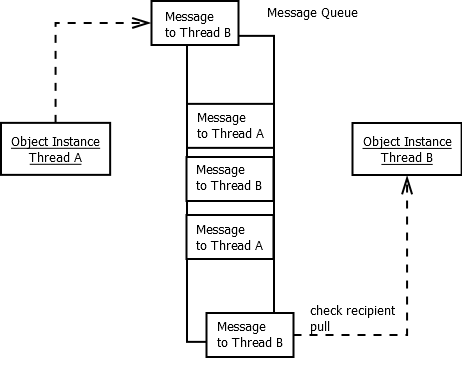
\includegraphics[width=0.8\textwidth]{img/MessageQueue.png}
  %  \caption{MessageQueue}
    \label{MessageQueue}
  \end{centering}
\end{figure}
Die Kommunikation mittels einer MessageQueue kann in zwei Formen realisiert werden:
\begin{itemize}
\item Unidirektional
\item Bidirektional
\end{itemize}
Bei der unidirektionalen Kommunikationsform darf ein Kommunikationspartner nur entweder Nachrichten aus der Queue entnehmen oder hinein geben. In unserem Beispiel dürfte demnach nur die Objekt Instanz des Thread A Nachrichten in die Queue geben und die Objekt Instanz des Thread B darf lediglich aus dieser lesen.\newline
Bei der bidirektionalen Kommunikationsform dürfen beide Kommunikationspartner je Nachrichten in die MessageQueue einstellen wie auch herausnehmen.\newline 
\newline

Die letzten beiden Abschnitte haben einen Überblick über Technologieen gegeben, mit denen der Austausch von Informationen innerhalb einer nebenläufigen Verarbeitung über Thread Grenzen hinaus realisiert werden kann. Dabei stellen MessageQueues eine Abstraktionsebene zur Kommunikation über fest definierten Speicher dar. Die Entwicklung von Nebenläufigkeit kann jedoch auch zu schwerwiegenden Problemen führen.


\section{Risiken von Nebenläufigkeit}
Der Botschaftenaustausch zwischen Threads, sowie deren Synchronisation kann zu schwerwiegenden Problemen im Zuge der Prallelverarbeitung führen. Folgende Szenarien sind eher allgemein gehalten, jedoch gilt es, besonders in dem Kapitel 2  zu den konkreten Implementierungen von Nebenläufigkeit, diese Problematiken zu beachten. In Kapitel 3 werden die in Kapitel 2 zu diskutierenden Beispielimplementierungen u.a. an Hand der hier aufgeführten Risikoszenarien und dem damit verbundenen Fehlerpotential bewertet.


\subsection{Philosophenproblem}
Ein zentrales Problem der theoretischen Informatik ist das Philosophenproblem das erstmals beschrieben wurde durch Edsger W. Dijkstra. Darin wird ein Szenario berschrieben, in dem eine bestimmte Anzahl von Philosophen auf begrenzte Ressourcen zugreifen und bei gleichzeitigem Zugriff sich gegenseitig blockieren können.

\begin{figure}[H]
  \begin{centering}
    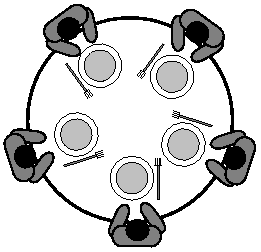
\includegraphics[width=0.6\textwidth]{img/PhilosophenProblem.png}
    \caption{Philosophenproblem \cite[vgl. ]{002}}
    \label{Philosophenproblem}
  \end{centering}
\end{figure}
Die Abbildung zeigt wie eine Gruppe von Philosophen an einem Runden Tisch sitzen, vor ihnen etwas zu Essen. Um zu essen, benötigen nach diesem theoretischen Aufbau die Philosophen die rechte und die linke Gabel neben dem jeweiligen Teller. Dabei versuchen die Philosophen zu nächst die Gabel zu ihrer Linken zu nehmen. Ist die Gabel frei, so behälten sie diese in der Hand bis auch die Gabel auf der rechten aufgenommen werden kann. Kann ein Philosoph eine Gabel zur Zeit nicht nehmen, da sie in Verwendung ist, verweilt er denkend bis die benötigte Gabel frei ist. Versuchen jedoch alle Philosophen gleichzeitig die Gabeln aufzunehmen, so besteht die Gefahr einer Verklemmung (engl. Deadlock). Der Ablauf stockt und die Philosophen verharren denkend bis sie verhungern. In Bezug auf die Kommunikation über geteilten Speicher oder Dateien kann dieses Problem auftreten wenn parallele Zugriffe auf exklusive Ressourcen nicht sauber synchronisiert werden.



\subsection{Race Conditions}
Ein weiteres Problem bei der Parallelverarbeitung tritt bei geteilten Speicher bzw. Daten auf. Folgende Abbildung illustriert das Szenario, dass drei Threads auf einen gemeinsamen Speicherbereich zugreifen. Die Threads eins bis drei greifen konkurrierend lesend, wie schreibend auf den Speicherbereich zu und tauschen darüber Informationen untereinander aus. Der Zugriff erfolgt nach dem Prinzip \glqq Wer zuerst kommt mahlt zuerst\grqq  ( = Race Condition).

\begin{figure}[H]
  \begin{centering}
    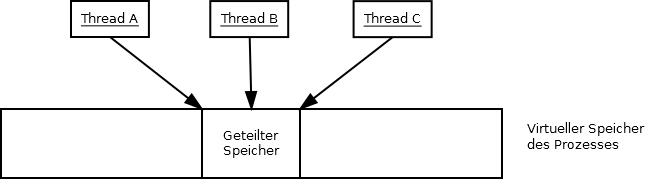
\includegraphics[width=0.8\textwidth]{img/SharedMemory_RaceCondition.png}
 %   \caption{Race_Condition beim Shared Memory  \cite[vgl. ]{002}}
    \label{SharedMemory_RaceCondition}
  \end{centering}
\end{figure}
Ist der Zugriff der Threads auf den Speicher nicht synchronisiert, so kommt es zu dem Shared Memory Effekt, (geteilter Speicher Effekt) nach dem eine Datenstruktur die, die Grundlage von Berechnungen darstellt, durch einen anderen Thread verändert wird, ohne dass die Änderung dem ersten Thread bekannt gemacht wird. Da solche Probleme von der jeweils in diesem Moment vorliegenden Prozessauslastung im System abhängen (tatsächlich gleichzeitig laufende Threads im Multi Core System), sind derartige Effekte schwer reproduzierbar und somit auch die Ursachen schwer zu finden.











\subsection{Resistive Touchbildschirm Technologie}
\begin{figure}[H]
  \begin{centering}
    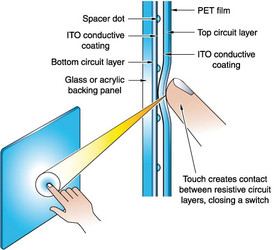
\includegraphics[width=0.8\textwidth]{img/Resistiv.png}
    \caption{Resistive Technologie \cite[vgl. Resistiv-4-5-7-und-8-Draht]{002}}
    \label{Resistiv}
  \end{centering}
\end{figure}
In der resistiven Touchscreen-Technologie wird ein Touchbildschirm in Deckschicht und Grundschicht unterteilt. An den Innenkanten beider Schichten ist ein leitender Film angebracht, der je mit unterschiedlicher Spannung geladen ist. Wie in der Abbildung gezeigt, schließt eine Berührung den Stromkreis und mit Hilfe der an den Bildschirmkanten angebrachten Sensoren die genauen Koordinaten des Berührungspunktes ermittelt. Prinzipiell ist bei dieser Technologie die Erkennung von Mehrfachberührungen möglich, jedoch hängt dies von den verbauten Sensoren ab.

\subsection{Surface Accustic Wave (SAW)}
\begin{figure}[H]
  \begin{centering}
    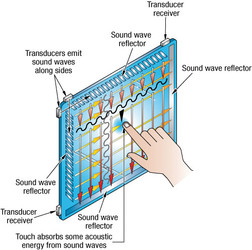
\includegraphics[width=0.8\textwidth]{img/surface_accustic_wave.png}
    \caption{Surface Accustic Wave Technologie \cite[vgl. Surface-Acoustic-Wave-Saw]{002}}
    \label{surface_accustic_wave}
  \end{centering}
\end{figure}
Das technische Prinzip dieser Technologie ist vergleichbar mit dem des Infrarot-Gitters. Schallwellen werden an bestimmten Punkten des Touchbildschirms emittiert und an zwei Kanten (x;y) so reflektiert, dass ein Raster durch die Schallwellen im Berührungsbereich aufgespannt wird. An den zwei übrigen Kanten leiten Reflektoren die einzelnen Schallwellen zu einem Sensor. Die Berührung hat eine Dämpfung der Schallwellen (in x- und y-Richtung) zur Folge, die zum Zeitpunkt der Berührung den Berührungspunkt passieren. Da die Schallwellen zeitverzögert erzeugt werden, also nur immer eine Schallwelle in eine X-Richtung und nur eine in Y-Richtung, ist somit der Berührungspunkt genau zu ermitteln. Dies bedeutet jedoch auch, dass zum selben Zeitpunkt nur ein Berührungspunkt ermittelbar ist, womit Multi-Touch-Gesten durch diese Technologie nicht unterstützt werden.

\subsection{Oberflächen-kapazitive Touchscreen Technologie}
\begin{figure}[H]
  \begin{centering}
    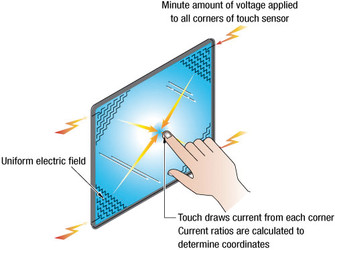
\includegraphics[width=0.8\textwidth]{img/oberflaechen_kapazitiv.png}
    \caption{Oberflächen Kapazitive Technologie}
    \label{oberflächen_kapazitiv}
  \end{centering}
\end{figure}
Die kapazitive Touchscreen-Technologie registriert Berührungen durch die Ablenkung innerhalb eines elektronischen Feldes, welches durch Elektroden an den Bildschirmkanten erzeugt wird. Sensoren an den Bildschirm-ecken messen dabei das elektronische Feld und damit jegliche durch Berührung ausgelöste Veränderung des Feldes. Der Finger fungiert dabei als Erdung, über den Elektronen aus dem Feld abfließen und somit für einen Spannungsabfall während der Berührung sorgt. Die genaue X- und Y- Koordinate errechnet sich aus den Strömen, die an den Sensoren registriert werden. Auch hier beschränkt sich die Technologie auf die Registrierung von lediglich einer Geste.


\subsection{Projiziert Kapazitiver Touchscreen Technologie}
\begin{figure}[H]
  \begin{centering}
    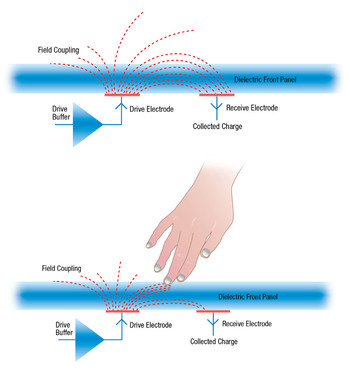
\includegraphics[width=0.8\textwidth]{img/projiziert_kapazitiv.png}
    \caption{Projiziert Kapazitive Technologie \cite[vgl. Projected-Capacitive]{002}}
    \label{projiziert_kapazitiv}
  \end{centering}
\end{figure}
Die projiziert- kapazitive Touchscreen-Technologie erweitert die Oberflächen-Kapazitiv-Technologie um einzelne kleinere Felder auf dem Touchbildschirm und ist die aktuellste der genannten Technologien. Der wesentliche Vorteil gegenüber der Oberflächen-Kapazitiven-Technologie ist, dass hier schon die Näherung eines Fingers ausreicht, um eine Berührung zu registrieren. Dadurch ist es möglich selbst durch dünne Handschuhe eine Berührung zu registrieren, was einen klassischen Einsatzkontext für den medizinischen Bereich darstellt. Die Abbildung zeigt, wie allein durch die Annäherung eines Fingers Teilbereiche des Feldes durch natürliche Ladung in den Fingern abgelenkt werden.

\chapter{Gestenerkennung und Steuerung von Funktionalität durch Gesten}
\section{Signalverarbeitung und erste Gesteninterpretation durch das Android OS}
Die Auflistung der einzelnen Technologien zum Touchbildschirm hat gezeigt, wie unterschiedlich die Umsetzungen der Berührungserkennung und deren Leistungsfähigkeit in Bezug auf die Erkennung von einfachen und mehrfachen Berührungen zur selben Zeit sind. Das Android Betriebssystem ist darauf ausgelegt, die unterschiedlichen Formen von Touchbildschirmen zu unterstützen. Je nach verbauter Technologie ist dabei die Erkennung von mehreren Berührungspunkten freigeschaltet oder nicht. Für den Entwickler einer Android Applikation ist dies jedoch völlig transparent. Im Falle einer registrierten Berührung wirft die API ein sogenanntes „MotionEvent“. Die Android API leistet hier eine erste Interpretation der Gesten, denn je nach Art der Berührung wird ein bestimmtes „MotionEvent“ gefeuert. Diese Events können abgefangen werden und liefern Berührungsparameter (Koordinaten) für eine weitere, detailliertere Interpretation der Gesten.
Der folgende Abschnitt beschreibt die prototypische Implementierung exemplarischer Gesten und geht neben den Besonderheiten und Schwierigkeiten der Gesteninterpretation auch auf die durch die Android API angebotenen MotionEvents ein.


\section{Erkennung und Interpretation von Gesten sowie Steuerung jeweiliger Funktionalität durch Gesten}
Für die Erkennung von Gesten bietet das Android SDK die Schnittstelle OnTouchListener an. Darin lässt sich die Methode\newline
   \centerline{ \texttt{boolean onTouch(View zoomView, MotionEvent anEvent)\{...\}}}\newline
überschreiben. Über den Parameter anEvent vom Typ MotionEvent können unterschiedliche Berührungsgesten erkannt werden. Die Methode OnTouchListener wird in Abhängigkeit von bestimmten Ereignissen aufgerufen. Hierzu ist zu einer View-Instanz die konkrete Implementierung des OnTouchListener Interfaces zu adressieren:\newline \centerline{\texttt{viewInstance.setOnTouchListener(touchListenerImpl);}}\newline
Wenn der Touchsensor eine Berührung registriert, wird für das jeweilige Layout geprüft, welche darin enthaltenen Views die Methoden des OnTouchListeners überschreiben und das Event an die jeweilige Implementierung weitergeleitet. Des Weiteren ist dem Objekt vom Typ MotionEvent zu entnehmen, um welche Art von Berührung es sich handelt.
Je nach Art und Weise der Berührung liefert die Maskierung der zur Event Aktion\newline
\centerline{\texttt{anEvent.getActionMasked()}}\newline\newline
ein Ergebnis, welches durch ein Element der Menge aus den folgenden Konstanten beschrieben wird:\newline
Menge M\newline
\{\newline\texttt{
   int ACTION\_DOWN = 0;\newline
   int ACTION\_UP = 1;\newline
   int ACTION\_MOVE = 2;\newline
   int ACTION\_CANCEL = 3;\newline
   int ACTION\_OUTSIDE = 4;\newline
   int ACTION\_POINTER\_DOWN = 5;\newline
   int ACTION\_POINTER\_UP = 6;\newline
   int ACTION\_HOVER\_MOVE = 7;\newline
   int ACTION\_SCROLL = 8;\newline
   int ACTION\_HOVER\_ENTER = 9;\newline
   int ACTION\_HOVER\_EXIT = 10;\newline}
\}\newline \newline
Für die Interpretation der Gesten und weiter die Steuerung exemplarischer Funktionalitäten wie Zoom oder Drag gilt dann:\newline\newline
ACTION\_DOWN: Der Touchsensor registriert eine Berührung in einem in sich geschlossenen Bereich.\newline
Beispiel: Die Fingerkuppe eines Nutzers berührt den Touchscreen. Die Koordinaten erhält der Entwickler durch das Auslesen des Event-Parameters. Über die Methoden\newline
\centerline{\texttt{anEvent.getX()} und}  \newline
\centerline{\texttt{anEvent.getY()}}\newline
können die Koordinaten ausgelesen werden, auf denen sich ein Finger auf dem Touchbildschirm befindet. Diese Methoden geben im Fall von mehrerer Berührungen (z.B. mehrere Finger) immer die Koordinaten des ersten Berührungspunktes an.\newline\newline
ACTION\_UP: Der Touchsensor registriert das Aufheben einer ursprünglich registrierten Berührung. Dies setzt zuvor die Registrierung einer ACTION\_DOWN voraus.\newline\newline
ACTION\_POINTER\_DOWN:
Der Touchsensor registriert eine zweite Berührung (zweiter Finger). Die Koordinaten der zweiten Berührung, sowie auch im Falle weiterer Berührungspunkte, lassen sich aus dem Event entsprechend der Reihenfolge der Berührung ermitteln:
\centerline{\texttt{anEvent.getX(0..n);}}\newline
\centerline{\texttt{anEvent.getY(0..n);}}\newline
Dies entspricht der Berührung mit dem ersten bis N-ten Finger. Für die Funktionalität Zoom ist es notwendig, die initiale Distanz zwischen den zwei Berührungspunkten zu ermitteln und temporär vorzuhalten.\newline\newline
ACTION\_MOVE: Der Touchsensor registriert eine Bewegung weg vom ursprünglich registrierten Berührungspunkt, dessen Ermittlung diesem Event vorausgeht. Um die o.g. Funktionalitäten zu realisieren, wird für die Ein-Finger-Geste "Drag" der Richtungsvektor bei einer Bewegung auf dem Touchbildschirm ermittelt, indem vom initialen Berührungsspunkt bis zur aktuellen Position des Fingers die Differenz in x wie in y Richtung errechnet wird.


\section{Gestengesteuertes Vergrößern und Verkleinern sowie Veränderung des Fokus für Darstellungsobjekte vom Typ ImageView}
Ian F. Darwin liefert mit seinem Kochbuch für die Android Entwicklung zu der Zoomfunktionalität folgenden Ansatz: \newline
\texttt{// Remember some things for zooming \newline
PointF start = new PointF();\newline\newline
ImageView view = (ImageView) v;\newline
// make the image scalable as a matrix \newline
view.setScaleType(ImageView.ScaleType.MATRIX);\newline
...\newline
switch (event.getAction() \& MotionEvent.ACTION\_MASK) \{ \newline
case MotionEvent.ACTION\_DOWN: //first finger down only\newline
start.set(event.getX(), event.getY());\newline
break;\newline
...\newline
case MotionEvent.ACTION\_MOVE:\newline
if (mode == DRAG)\newline
matrix.postTranslate(event.getX() - start.x, event.getY() - start.y);\newline
\newline
else if (mode == ZOOM)\newline
matrix.postScale(scale, scale, mid.x, mid.y);\newline
\newline
// Perform the transformation\newline
view.setImageMatrix(matrix);\newline
\} \newline 
}\cite[S. 234-237.]{003}\newline
Diese Auszüge aus Darwins Kochbuch zur Andorid Entwicklung zeigen schematisch die dynamische Skalierung einer ImageView in Abhängigkeit der erkannten Gesten mit Hilfe einer speziell für diesen Objekttyp anpassbaren Matrix. Die Matrix lässt sich direkt aus einer Objektinstanz vom Typ ImageView holen und mittels der Methoden
\begin{itemize}
\item \texttt{postTranslate()} und
\item \texttt{postScale()}
\end{itemize}
verarbeiten. Dabei ist zu beachten, dass die Matrix nicht direkt verändert werden darf, sondern nur deren Kopie. Der Richtungsvektor für die neue Fokussierung und damit Transformation der Matix errechnet sich aus der Differenz der aktuellen Koordinaten zu den Anfangskoordinaten und wird zur Transformation der Matrix entsprechend übergeben:\newline
\centerline{ \texttt{ matrix.postTranslate(event.getX() - start.x,}} \newline \centerline{ \texttt{ event.getY() - start.y) }}\newline \newline
Im Fall von mehreren registrierten Berührungen, wie z.B. bei der Pinch-Open-Geste für die Ansteuerung einer Zoom-Funktionalität, muss zunächst die Anfangsdistanz zwischen den Berührungspunkten auf dem Touchbildschirm ermittelt werden. In einem Koordinatensystem aus zwei Dimensionen (x|y) wird die Länge einer Strecke von P1(xp1|yp1) und P2(xp2|yp2) wie folgt berechnet:
\centerline{$\sqrt{(x_{0}-x_{1})^{2}+(y_{0}-y_{1})^{2}}$ }\newline\newline
In Darwins Implementierung ist dies in der Methode \texttt{spacing()} realisiert. Weiter ist über das gesamte ACTION\_MOVE Event hinweg, die neue Distanz der Berührungspunkte zu berechnen und mit der initialen Distanz in ein Verhältnis zu setzen. Der Quotient aus
\centerline{$ ScaleFaktor = \dfrac{dist_{new}}{dist_{old}}$} \newline\newline
ergibt den Faktor für die Skalierung der ImageView. Die ImageView wird daraufhin entsprechend relativ zu der Positionsänderung der Berührungspunkte neu skaliert.\newline
\centerline{ \texttt{ matrix.postScale(scale, scale, mid.x, mid.y);}} \newline\newline
Darwins Vorgehensweise stellt eine komfortable und einfache Möglichkeit dar, eine ImageView Instanz dynamisch zu skalieren oder den Fokus der Darstellung zu verändern. Jedoch bezieht sich die Lösung allein auf Darstellungselemente vom Typ ImageView, wohingegen die Superklasse View, die durch ImageView erweitert wird, es nicht vorsieht die Matrix zur Skalierung und Positionierung der View direkt zu verändern. Damit ist Darwins Lösung allein für Darstellungsobjekte vom Typ ImageView geeignet.

\section{Abstraktion gestengesteuerter Funktionalitäten zum Skalieren und Fokussieren von Darstellungselementen}
Dieser Abschnitt beschäftigt sich mit der Frage, inwieweit sich der Ansatz von Darwin generalisieren lässt und somit unabhängiger vom Typ des Darstellungsobjektes wird. Kann hierzu eine Lösung gefunden werden, so ist weitergehend zu diskutieren, inwieweit diese für andere Android App Projekte verfügbar gemacht werden kann.

\subsection{Generalisierung der Funktionalitäten zum Skalieren und Fokussieren von Darstellungselementen}
Die skizzierte Implementierung nach I.F. Darwin im letzten Abschnitt zeigt zwar, wie ein bestimmtes Darstellungselement in Abhängigkeit von bestimmten Gesten skaliert, jedoch gilt diese Lösung nicht für andere Darstellungselemente. Ein generischer Ansatz müsste die Skalierung und Fokussierung für alle Darstellungselemente leisten, mindestens jedoch für alle Elemente, die vom Typ android.view.View ableiten.\newline
Der im Folgenden skizzierte Prototyp soll Darwins Ansatz um eine dynamische Anzahl von Darstellungselementen mit der Kompatibilität zu unterschiedlichen Darstellungstypen erweitern.
Dieser Projektarbeit liegt eine prototypische Implementierung bei (Klasse \texttt{Touch.java}), in der das Skalieren und Fokussieren von Darstellungselementen für allgemein alle Objekte ermöglicht wird, die vom Typ \texttt{android.view.View} ableiten (z.B. \texttt{TextView extends View}). Ein entsprechender Algorithmus könnte damit die Funktionalität zur Skalierung und Fokussierung applikationsübergreifend generalisieren. 
Für die Skalierung eines Darstellungsobjektes vom Typ View bietet die Android API folgende Methoden an:
\begin{itemize}
\item \texttt{setScaleX()}
\item \texttt{setScaleY()}
\end{itemize}
und für die Veränderung des Fokus auf die View:
\begin{itemize}
\item \texttt{setTranslationX()}
\item \texttt{setTranslationY()}
\end{itemize}
Ein dabei auftretendes Problem sind unerwünschte Seiteneffekte bei der Verwendung des Listeners zur Registrierung von Berührungen und Bewegungen. Dieser Listener kann einer View zugeordnet werden:
\centerline{\texttt{viewInstance.setOnTouchListener(touchListenerInstance)}}\newline \newline
Wird jedoch dieselbe View-Instanz innerhalb der TouchListener-Implementierung neu skaliert, kommt es auf Grund der angestoßenen Zoom-Funktionalität zu einem flackernden Übergang von der ursprünglichen Skalierung in die neue Skalierung. Dies liegt daran, dass das Koordinatensystem der View durch die Skalierung unmittelbar selbst verändert wird. Stellt diese View jedoch auch das Koordinatensystem für die Gestenerkennung, (\texttt{viewInstance.setOnTouchListener(...)}), so wird die Berechnung des Zoomfaktors gestört.
 \newline
Die View, welche durch den Zoom neu skaliert wird, darf also im Falle einer gestengetriebenen Zoom-Funktionalität nie die Bemessungsgrundlage (Koordinaten) für die Berechnung des Skalierungsfaktors sein. Alternativ kann die sogenannte Parent-View der zu skalierenden View-Instanz als Bemessungsgrundlage herangezogen werden, wie es die folgende Abbildung zeigt: \newline
\begin{figure}[H]
  \begin{centering}
    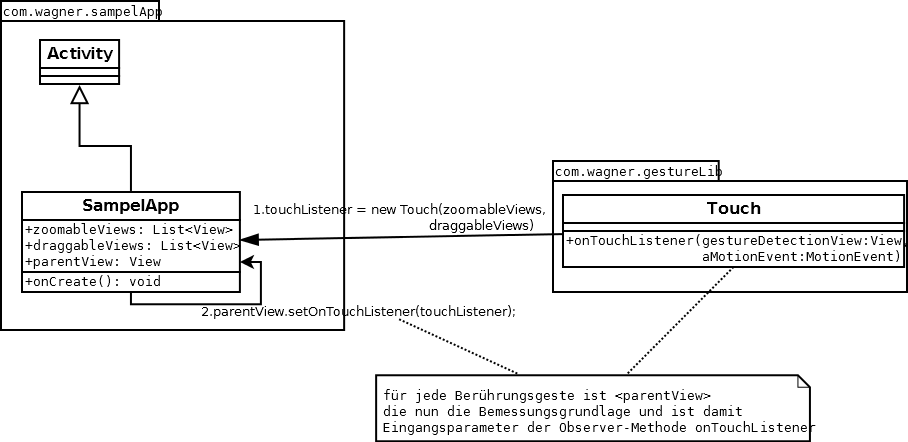
\includegraphics[width=0.8\textwidth]{img/touchFragments.png}
    \caption{Konzeption eines generischen Touchlisteners}
    \label{callingTouchListener}
  \end{centering}
\end{figure} Die Parent-View ist in der Baumstruktur des Layouts einer View- Instanz übergeordnet. 

\subsection{Ausblick zur Integration der generischen Implementierung zu gestengesteuerten Funktionalitäten}
Der letzte Abschnitt hat gezeigt, wie gestengesteuerte Funktionalitäten zum Skalieren und Fokussieren von Darstellungselementen, allgemein für unterschiedliche Darstellungstypen definiert werden können. Dieser Abschnitt gibt einen Ausblick, wie der entworfene Ansatz aus dem letzten Kapitel allgemein für Android Applikationsprojekte angeboten werden kann.\newline
In Android Projekten lassen sich wie auch in anderen Java Projekten zusätzliche Bibliotheken in Form von .jar - Archiv Dateien einbinden. Grundsätzlich ist es möglich diese Bibliotheken manuell in die jeweilige Entwicklungsumgebung einzufügen. Sollten jedoch unterschiedliche Versionen zu den jeweiligen Android APIs unterschieden werden sind bestimmte Werkzeuge zur Versionverwaltung und dem übersichtlichen Management von Abhängigkeiten zu empfehlen. Auch wenn Tests zu Funktionalitäten der Bibliothek vor dem Erzeugen des .jar - Archives durchlaufen werden müssen, sollte dies automatisiert sein. Hierzu gibt es unterschiedliche Werkzeuge, die sich für das Auflösen von Abhängigkeiten sowie das finale Bauen der Applikation anbieten. Exemplarisch bietet sich hier das Build Werkzeug \glqq Maven\grqq mit dem Android Plugin an. Der im letzten Kapitel entworfene Ansatz lässt sich damit in eine eigenständige Bibliothek auslagern, um diesen in unterschiedlichen Android-Applikationsprojekten zu nutzen.

\section{Fazit}
Eingangs stand die Frage im Raum, wie den Einstiegshürden in der Android-Entwicklung sowie dem Problem des Code-Copy entgegen gewirkt werden kann. Anhand der Entwicklung von gestengesteuerter Funktionalität (speziell hier Zoom und Drag) ist verdeutlicht worden, welche Schwierigkeiten auf Einsteiger in der Android Entwicklung warten. Gleichzeitig wird mit der Implementierung nach Darwin (Kapitel 3.3) deutlich, welche Mengen an komplexem Sourcecode zu gestengesteuerter  Funktionalität (siehe Implementierung nach F.Darwin Kapitel 3.3) in Applikationsprojekte integriert werden müsste, um grundlegendes Verhalten zu definieren. Der in diesem Projekt geschaffene Ansatz zur Generalisierung von gestengesteuerter Funktionalität bietet die Möglichkeit den dahinterstehenden Programmcode zu zentralisieren, also Code Copy vorzubeugen und gleichzeitig die Android App-Entwicklung zu vereinfachen.
Für weitere gestengesteuerte Funktionalitäten kann ähnlich verfahren werden, vorausgesetzt es kann ein geeigneter Abstraktionsgrad gefunden werden, wie er hier für die Skalierung und Fokussierung definiert ist.

\bibliography{Praxisprojekt}{}
\bibliographystyle{jureco} %% jurabib, jureco, jurunsrt, 
%% \printindex

\appendix

\chapter*{Anhang}
 \lstinputlisting
    [caption={Die Klasse Touch.java}
       \label{lst:javaclass},
       captionpos=t,language=JAVA]
 {listings/Touch.java}
\addcontentsline{toc}{chapter}{Anhang}
\chapter{Erklärung}

Ich versichere, die von mir vorgelegte Arbeit selbständig verfasst zu
haben. Alle Stellen, die wörtlich oder sinngemäß aus veröffentlichten
oder nicht veröffentlichten Arbeiten anderer entnommen sind, habe ich
als entnommen kenntlich gemacht. Sämtliche Quellen und Hilfsmittel,
die ich für die Arbeit benutzt habe, sind angegeben. Die Arbeit hat
mit gleichem Inhalt bzw. in wesentlichen Teilen noch keiner anderen
Prüfungsbehörde vorgelegen.

\bigskip

Gummersbach, den \today

\bigskip

\bigskip

\bigskip

\bigskip

\bigskip

\bigskip

(Unterschrift)

\end{document}

%% end of file
